\documentclass[12pt]{article}

% Package Imports
\usepackage{amsmath,amssymb}
\usepackage{graphicx}
\usepackage[margin=1in]{geometry}
\usepackage{setspace}
\usepackage{authblk}
\usepackage{caption}
\usepackage{subfigure}
\usepackage[numbers, sort]{natbib}

% Title and Author Setup (same as main)
\title{quantms-rescoring and multi-engine searching enable deep proteome coverage across quantitative proteomics, immunopeptidomics, and phosphoproteomics}
\author[1,2]{Chengxin Dai}
\author[3,4]{Ralf Gabriels}
\author[3,4]{Robbin Bouwmeester}
\author[5,6,7,8]{Jonas Scheid}
\author[9]{Henry Webel}
\author[3,4,10,11]{Lennart Martens}
\author[11]{Oliver Kohlbacher}
\author[12]{Mingze Bai}
\author[13]{Timo Sachsenberg}
\author[14,$*$]{Yasset Perez-Riverol}
\affil[1]{State Key Laboratory of Medical Proteomics, Beijing Proteome Research Center, National Center for Protein Sciences (Beijing), Beijing Institute of Lifeomics, 102206, Beijing, China}
\affil[2]{International Academy of Phronesis Medicine (Guangdong), 510320, Guangdong, China}
\affil[3]{CompOmics, VIB Center for Medical Biotechnology, VIB, Ghent, 9052, Belgium}
\affil[4]{Department of Biomolecular Medicine, Faculty of Medicine and Health Sciences, Ghent University, Ghent, 9052, Belgium}
\affil[5]{Department of Peptide-based Immunotherapy, Institute of Immunology, University and University Hospital Tübingen, Tübingen, Germany}
\affil[6]{Cluster of Excellence iFIT (EXC2180) Image-Guided and Functionally Instructed Tumor Therapies, University of Tübingen, Tübingen, Germany}
\affil[7]{Quantitative Biology Center (QBiC), University of Tübingen, Tübingen, Germany}
\affil[8]{Institute for Bioinformatics and Medical Informatics (IBMI), University of Tübingen, Tübingen, Germany}
\affil[9]{The Novo Nordisk Foundation Center for Biosustainability, Technical University of Denmark, Lyngby, Denmark}
\affil[10]{BioOrganic Mass Spectrometry Laboratory (LSMBO), IPHC UMR 7178, University of Strasbourg, CNRS, Strasbourg, 67000, France}
\affil[11]{Infrastructure Nationale de Proteomique ProFI - FR2048, Strasbourg, 67087, France}
\affil[12]{Chongqing Key Laboratory of Big Data for Bio Intelligence, Chongqing University of Posts and Telecommunications, Chongqing, China}
\affil[13]{Department of Computer Science, Applied Bioinformatics, University of Tübingen, Tübingen, Germany}
\affil[14]{European Molecular Biology Laboratory, European Bioinformatics Institute, Wellcome Genome Campus, Cambridge, United Kingdom}
\affil[ ]{$*$Corresponding author: yperez@ebi.ac.uk}
\date{}

\begin{document}
\maketitle
\doublespacing

% Supplementary Figures
\renewcommand\thefigure{S\arabic{figure}}
\setcounter{figure}{0}

\begin{figure}[ht!]
\centering
\includegraphics[width=1\textwidth]{figures//LFQ_weights.png}
\caption{The weights that Percolator assigns to different features of the search engine feature vector in MSGF+ (A), Comet (B), and SAGE (C) combined with Percolator settings from PXD001819. The more different from zero a weight is (both positive and negative), the more important that feature is in the final Percolator classification.}
\label{fig:PXD001819_svm_weights}
\end{figure}

\begin{figure}[ht!]
\centering
\includegraphics[width=1\textwidth]{figures//CPTAC_weights.png}
\caption{The top 20 normalized weights from Percolator for MSGF+ (A), Comet (B), and SAGE (C) identification results from PDC000125.}
\label{fig:PDC_ms2rescore_weights}
\end{figure}

\begin{figure}[ht!]
\centering
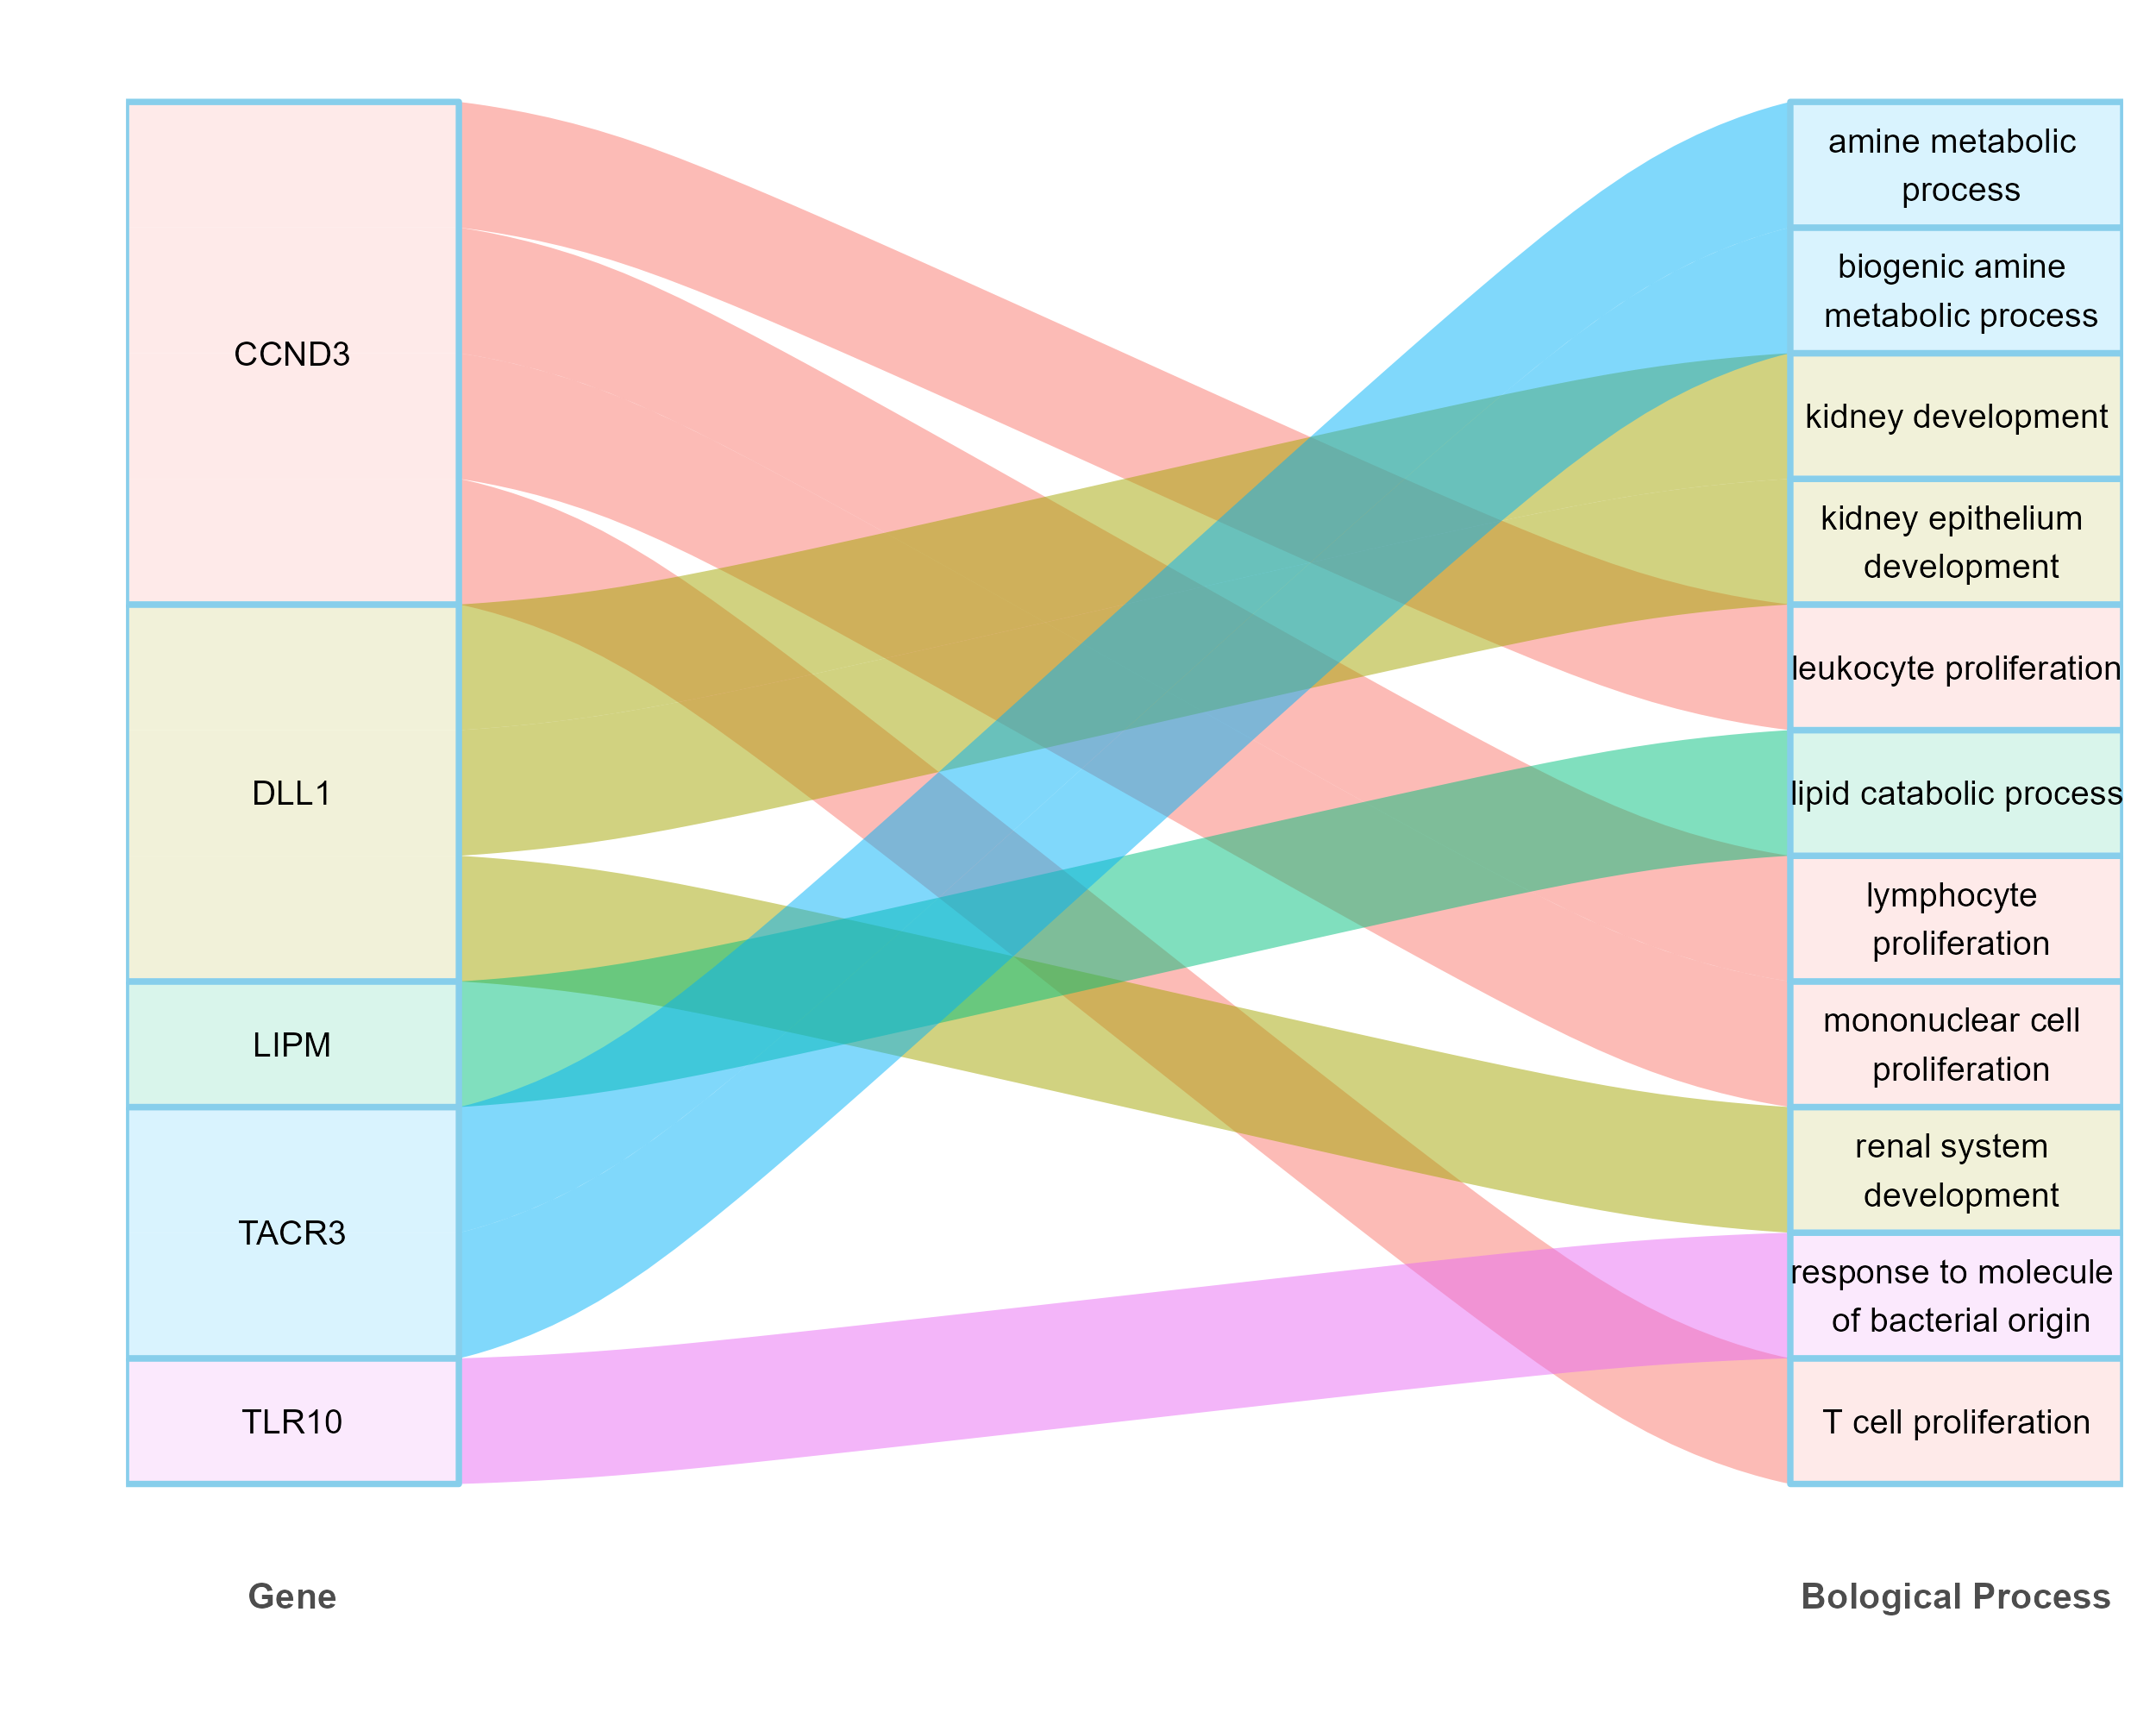
\includegraphics[width=1\textwidth]{figures//ego_results_alluvial.png}
\caption{The GO enrichment analysis for MSGF+\&Comet with quantms-rescoring. The Sankey diagram shows biological process term of the genes are uniquely reported by MSGF+\&Comet with quantms-rescoring compared without quantms-rescoring.}
\label{fig:PDC_Go_EA}
\end{figure}

\begin{figure}[ht!]
\centering
\includegraphics[width=1\textwidth]{figures//PXD019643.png}
\caption{Comparison of immunopeptides identification results for different workflow settings on PXD019643. (A) Line plot showing the number of spectra identified for four workflow settings at different PSM FDR levels. (B) Percentage of unique identified peptides using different workflow settings. Density plots showing the distribution of the smallest retention time error between observed and predicted retention time (C) and the Pearson correlation between observed and predicted peak intensities (D) for each PSM split into decoys (red), rejected targets with q-value $>$0.01 (blue), and accepted targets from individual support and consensus support with q-value $<$0.01 (green). Note that the rejected target distribution coincides with the decoy distribution. The pronounced spike at Pearson correlation = 0 reflects spectrum comparisons in which all predicted or observed peaks have zero intensity, causing a division-by-zero situation that leaves the Pearson correlation undefined.}
\label{fig:PXD019643_immunopeptides}
\end{figure}

\begin{figure}[ht!]
\centering
\includegraphics[width=1\textwidth]{figures//PXD019643_weights.png}
\caption{The top 20 normalized weights from Percolator for MSGF+ (A) and Comet (B) identification results in the PXD019643 dataset.}
\label{fig:PXD019643_features}
\end{figure}

\begin{figure}[ht!]
\centering
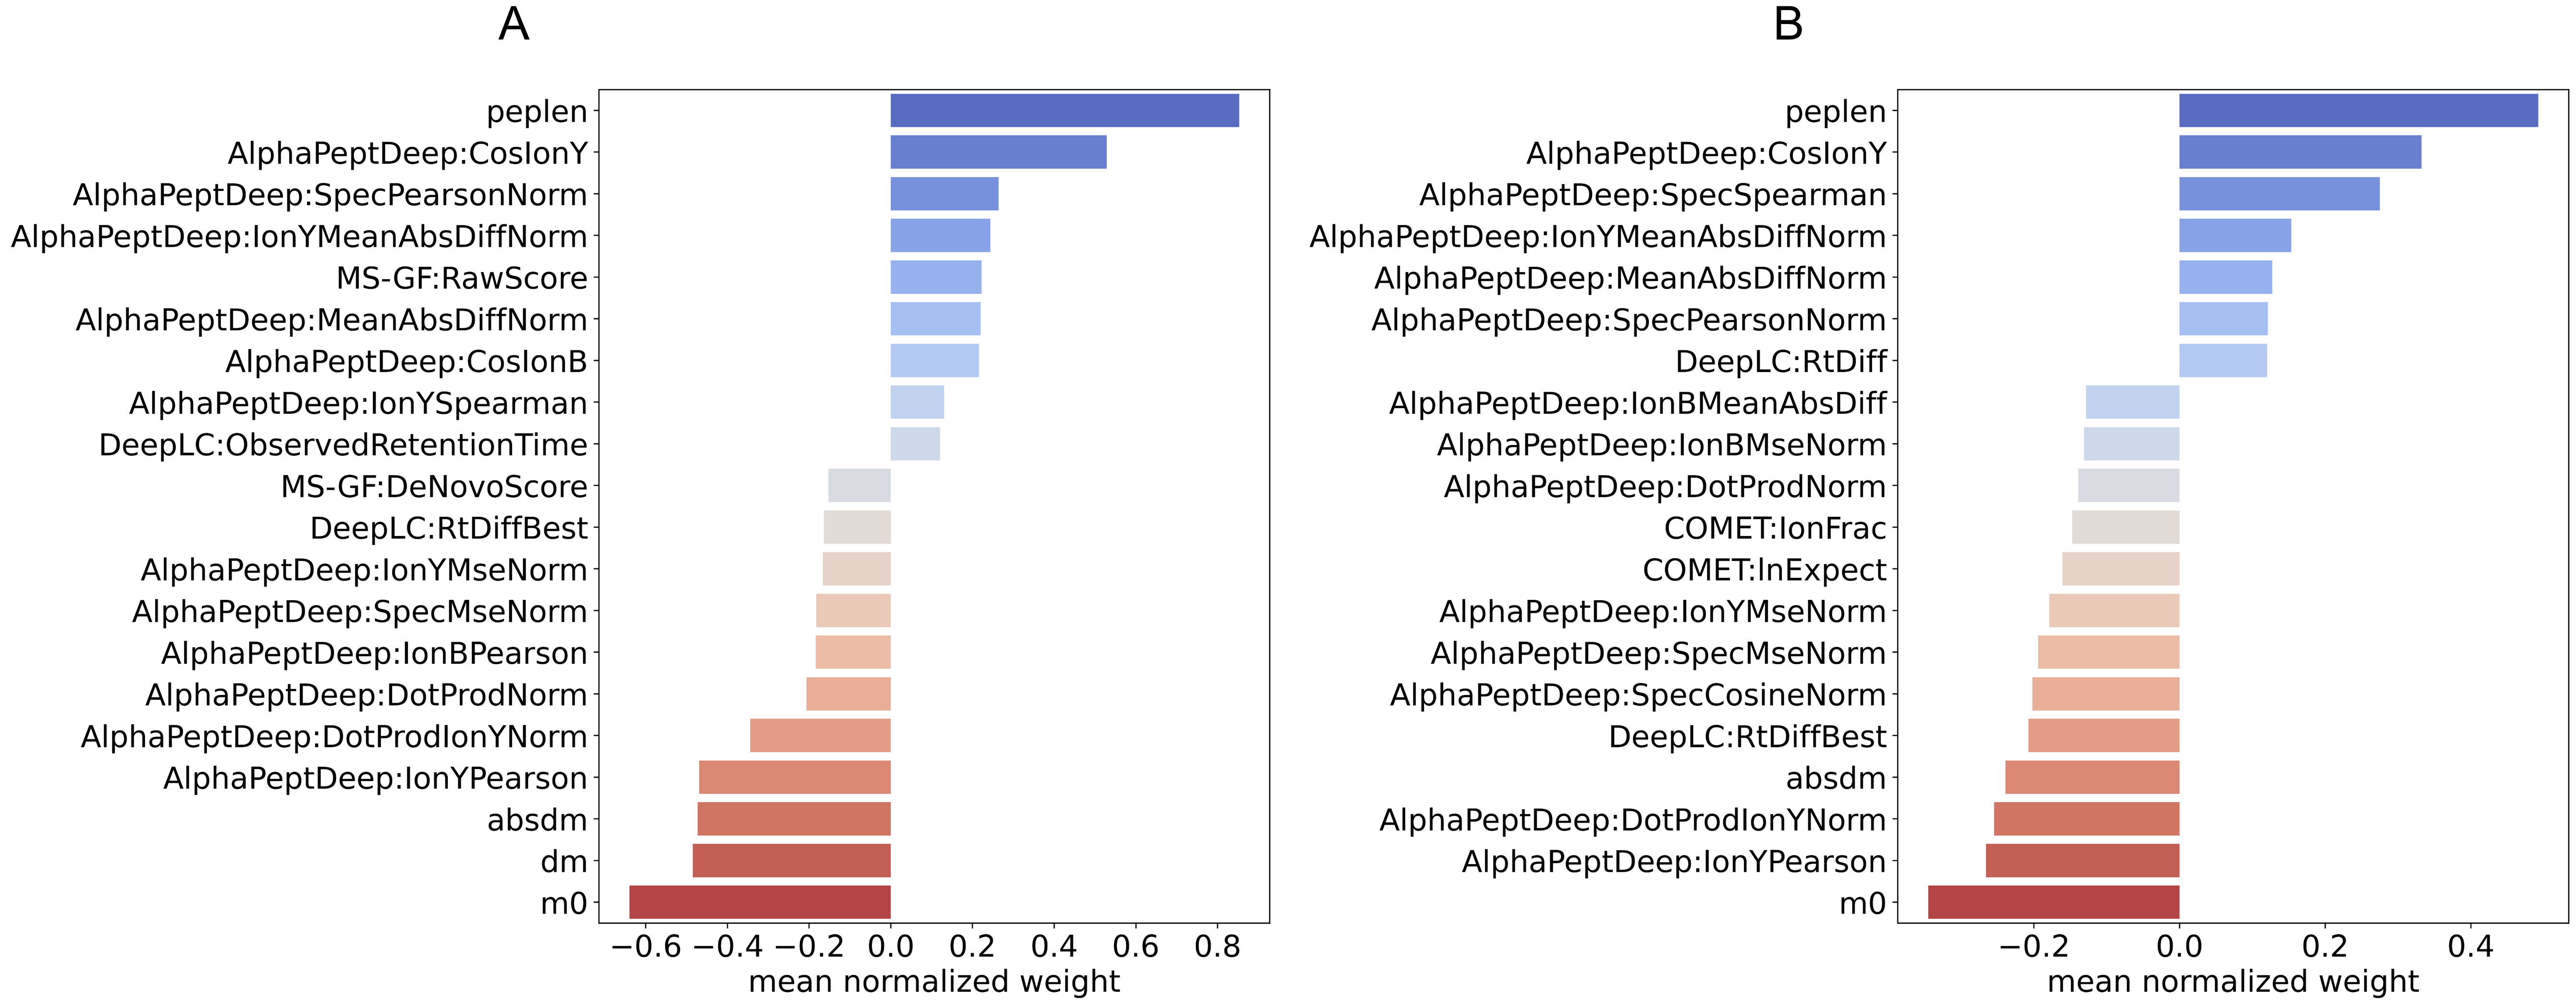
\includegraphics[width=1\textwidth]{figures//phos_peptdeep_weights.png}
\caption{The top 20 normalized weights from Percolator for MSGF+ (A) and Comet (B) identification results in the PXD026824 dataset.}
\label{fig:phospho_features}
\end{figure}

% Supplementary Tables
\renewcommand\thetable{S\arabic{table}}
\setcounter{table}{0}

\begin{table}[h!]
\centering
\caption{Spectrum-quality features. The memory and CPU values represent the maximum resources required for a single job. The quantms workflow was run in a 64 cluster queue.}
\begin{tabular}{|p{3.5cm}|p{10cm}|}
\hline
\textbf{Features} & \textbf{Definition} \\
\hline
signal to noise & The signal-to-noise ratio calculated as the maximum intensity divided by the root mean square deviation of the intensities for a spectrum. \\
\hline
spectral entropy  & The entropy of normalized intensity\\
\hline
fraction tic top 10 & The intensity fraction of top 10 peaks for total ion current\\
\hline
weighted std mz & The standard deviation of weighted m/z  \\
\hline
\end{tabular}
\label{tab:extra_features}
\end{table}

\begin{table}[h!]
\centering
\caption{Runtime, memory, and CPU consumption for different configurations. The memory and CPU values represent the maximum resources required for a single job. The quantms workflow was run in a 64 cluster queue.}
\begin{tabular}{|c|c|c|c|c|}
\hline
Datasets & Configuration & Runtime& Memory & CPU \\
\hline
PDC000127 & Comet\&MSGF+\&MS²Rescore & 9h39m & 30G & 7 \\
PDC000127 & Comet\&MSGF+ & 6h28m & 8G & 4 \\
PDC000127 & Comet & 5h10m & 8G & 4 \\
PXD019643 & Comet\&MSGF+\&MS²Rescore & 15h57m & 20G & 8 \\
PXD019643 & Comet\&MSGF+ & 13h09m & 5.5G & 4 \\
PXD019643 & Comet & 2h05m & 5.5G & 4 \\
PXD026824 & Comet\&MSGF+\&MS²Rescore & 2h05m & 66G & 8 \\
PXD026824 & Comet\&MSGF+ & 1h17m & 48.4G & 4 \\
PXD026824 & Comet & 24m & 48.4G & 4 \\
\hline
\end{tabular}
\label{tab:resources_stats}
\end{table}

\end{document}

